\documentclass[11pt,a4paper]{article}

\usepackage[utf8]{inputenc}
\usepackage[margin=2.5cm]{geometry}
\usepackage{amsmath,amssymb,amsthm,mathtools}
\usepackage{booktabs,tabularx,enumitem}
\usepackage{xcolor}
\usepackage{tikz}
\usetikzlibrary{arrows.meta,calc,patterns,positioning}
\usepackage{pgfplots}
\pgfplotsset{compat=1.18}
\usepackage[most]{tcolorbox}
\usepackage[colorlinks=true,linkcolor=blue!50!black,urlcolor=blue!50!black,citecolor=blue!50!black]{hyperref}
\usepackage[font=small,labelfont=bf]{caption}
\usepackage{float}

\setlength{\parindent}{0pt}
\setlength{\parskip}{5pt}
\setlist{itemsep=2pt,topsep=3pt}

% ---------- macros ----------
\newcommand{\Cspace}{\mathcal{C}}
\newcommand{\Wspace}{\mathcal{W}}
\newcommand{\Cfree}{\mathcal{C}_{\mathrm{free}}}
\newcommand{\CO}{\mathcal{CO}}
\newcommand{\Obs}{\mathcal{O}}
\newcommand{\Rob}{\mathcal{B}}
\newcommand{\Vor}{\mathcal{V}}
\newcommand{\R}{\mathbb{R}}
\newcommand{\vq}{\boldsymbol{q}}
\newcommand{\qs}{\boldsymbol{q}_s}
\newcommand{\qg}{\boldsymbol{q}_g}
\newcommand{\Mink}{\oplus}
\DeclareMathOperator{\card}{card}

\newcommand{\slides}[1]{\emph{(slides #1)}}
\newcommand{\sect}[2]{\section{#1\texorpdfstring{\ \slides{#2}}{ (slides #2)}}}
\newcommand{\subsect}[2]{\subsection{#1\texorpdfstring{\ \slides{#2}}{ (slides #2)}}}

% ---------- boxed theorem-like environments ----------
\tcbset{boxstyle/.style={enhanced,breakable,boxrule=0.6pt,arc=2pt,left=6pt,right=6pt,top=4pt,bottom=4pt,before skip=8pt,after skip=8pt}}

\theoremstyle{definition}
\newtheorem{definition}{Definition}[section]
\newtheorem{example}[definition]{Example}
\newtheorem{algorithm}[definition]{Algorithm}
\theoremstyle{plain}
\newtheorem{theorem}[definition]{Theorem}
\newtheorem{lemma}[definition]{Lemma}
\newtheorem{proposition}[definition]{Proposition}
\newtheorem{corollary}[definition]{Corollary}
\theoremstyle{remark}
\newtheorem{remark}[definition]{Remark}

\tcolorboxenvironment{definition}{boxstyle,colback=black!3,colframe=black!65}
\tcolorboxenvironment{theorem}{boxstyle,colback=red!4,colframe=red!60!black}
\tcolorboxenvironment{lemma}{boxstyle,colback=orange!5,colframe=orange!75!black}
\tcolorboxenvironment{proposition}{boxstyle,colback=orange!5,colframe=orange!75!black}
\tcolorboxenvironment{corollary}{boxstyle,colback=orange!5,colframe=orange!75!black}
\tcolorboxenvironment{example}{boxstyle,colback=teal!5,colframe=teal!65!black}
\tcolorboxenvironment{algorithm}{boxstyle,colback=violet!4,colframe=violet!65!black}

\newtcolorbox{intuition}{enhanced,colback=blue!5,colframe=blue!65!black,coltitle=white,
  fonttitle=\bfseries\sffamily,title=Intuition,boxrule=0.6pt,arc=3pt,left=6pt,right=6pt,top=3pt,bottom=3pt,
  before skip=8pt,after skip=10pt}

% ---------- placeholder for figures to be inserted by hand ----------
\newcommand{\figplaceholder}[2]{%
  \begin{center}
  \fcolorbox{red!70!black}{yellow!12}{\parbox[c][#1][c]{0.88\textwidth}{\centering
    \textbf{[\,INSERT IMAGE HERE\,]}\\[3pt] \small #2}}
  \end{center}}

\title{\textbf{Autonomous and Mobile Robotics}\\[4pt]\Large Motion Planning --- Introduction and Roadmap Methods}
\author{Lecture notes on Prof.\ G.\ Oriolo's lecture\\ Sapienza Universit\`a di Roma}
\date{\today}

\begin{document}
\maketitle
\tableofcontents
\bigskip

% =====================================================================
\sect{Introduction and Motivation}{2}
% =====================================================================

In the earlier parts of the course we learned how to design a feasible path or trajectory in a \emph{free} space, i.e.\ we implicitly assumed that nothing was in the robot's way. In practice, robots are expected to perform tasks in workspaces populated by physical objects that act as \emph{obstacles} to their motion. This chapter shows how to deal with them.

It also introduces a second major change: \textbf{autonomy}. An autonomous robot must be able to plan, by itself, a collision-free motion from an initial to a final posture, using

\begin{enumerate}[label=(\arabic*)]
  \item a high-level description of the task (e.g.\ ``go to the charging station''), and
  \item geometric information about the workspace.
\end{enumerate}

How the second ingredient becomes available splits the problem into two flavours.

\begin{definition}[Off-line and on-line planning]
In \emph{off-line planning} the information about the workspace geometry is entirely provided in advance (e.g.\ a complete map); the plan can be computed before the robot moves. In \emph{on-line planning} the information is gradually gathered by the robot through its own sensors while it moves; the robot starts, for instance, from an empty map and discovers the obstacles as it explores.
\end{definition}

\begin{intuition}
Off-line planning is like planning a route on a paper map of the city before leaving home. On-line planning is like finding your way through an unknown building in the dark with a torch: you can only react to what the torch lights up, and exploration of the workspace becomes part of the problem.
\end{intuition}

% =====================================================================
\sect{The Canonical Motion Planning Problem}{3--4}
% =====================================================================

To capture the intrinsic complexity of motion planning in a workspace with obstacles, we first define a clean ``canonical'' version of the problem; the algorithms of this chapter solve it, and the extensions are discussed afterwards.

\begin{definition}[Canonical motion planning problem]
\label{def:canonical}
Consider
\begin{itemize}
  \item a robot $\Rob$ (a single-body mobile robot, a kinematic chain with fixed base, or a kinematic chain with mobile base) moving in a workspace $\Wspace=\R^N$, with $N=2$ or $3$;
  \item obstacles $\Obs_1,\dots,\Obs_p$: fixed rigid objects in $\Wspace$ whose position and shape are known;
  \item $\Rob$ \emph{free-flying} in its configuration space $\Cspace$, i.e.\ not subject to kinematic constraints of any kind.
\end{itemize}
Given a start configuration $\qs$ and a goal configuration $\qg$ of $\Rob$ in $\Cspace$, plan a path that connects $\qs$ to $\qg$ and is \emph{safe}, i.e.\ it does not cause a collision between the robot and the obstacles. If no such path exists, report a failure.
\end{definition}

\begin{remark}[Names]
For a single-body robot in $\R^2$ the canonical problem is the \emph{piano movers' problem}; for a single-body robot in $\R^3$ it is the \emph{generalized movers' problem}.
\end{remark}

The canonical problem is \emph{purely geometric}: it asks for a collision-free \emph{path}, not for a trajectory with timing, and it ignores velocity or dynamic limits.

\begin{intuition}
The canonical problem is the ``spherical cow'' of motion planning: remove everything except geometry (known static obstacles, a robot that can go anywhere in $\Cspace$ that is not blocked). The point is to isolate the hard part---reasoning about free space---so that practical needs can be added afterwards as modifications of a method that already works.
\end{intuition}

\paragraph{Extensions to the canonical problem.} Each relaxes one assumption:
\begin{itemize}
  \item \textbf{moving obstacles} (people, other robots, cars, \dots);
  \item \textbf{on-line planning} (unknown environments);
  \item \textbf{kinematic constraints} (e.g.\ the nonholonomic constraints of wheeled robots);
  \item \textbf{manipulation planning}, which requires \emph{contact}: in the canonical problem even a simple touch counts as a collision, whereas in pick-and-place the robot must touch the grasped object (a ``controlled collision'').
\end{itemize}
Many methods that solve the canonical problem can be appropriately modified to address one or more of these extensions.

% =====================================================================
\sect{Obstacles in Configuration Space}{5--12}
% =====================================================================

\subsect{From the workspace to the configuration space}{5--6}

Planning directly in the workspace $\Wspace$ is hard: the robot is made of infinitely many points, so one would have to check collisions for each of them (and looking only at a point of interest such as the end effector is not enough). In the configuration space $\Cspace$ the robot is a \emph{single point}, and planning looks simpler: connect two points. What is missing is a representation of the obstacles in $\Cspace$, so we first define the \emph{image} of the obstacles there.

\begin{definition}[Volume occupied by the robot]
Let $\Rob(\vq)\subset\Wspace$ be the volume (exact region) of $\Wspace$ occupied by the robot when it is at configuration $\vq$.
\end{definition}

\begin{definition}[$\Cspace$-obstacle and $\Cspace$-obstacle region]
The image of the obstacle $\Obs_i$ in $\Cspace$ is the $i$-th \emph{$\Cspace$-obstacle}
\[
  \CO_i=\{\vq\in\Cspace:\ \Rob(\vq)\cap\Obs_i\neq\emptyset\}.
\]
The union of all the $\Cspace$-obstacles is the \emph{$\Cspace$-obstacle region}
\[
  \CO=\bigcup_{i=1}^{p}\CO_i .
\]
\end{definition}

\begin{definition}[Free configuration space and safe path]
The complement of $\CO$ is the \emph{free configuration space}
\[
  \Cfree=\Cspace-\CO=\Bigl\{\vq\in\Cspace:\ \Rob(\vq)\cap\Bigl(\bigcup_{i=1}^{p}\Obs_i\Bigr)=\emptyset\Bigr\}.
\]
A configuration-space path $\tau:[0,1]\to\Cspace$ is \emph{safe} (or \emph{free}) if and only if it belongs entirely to $\Cfree$, i.e.\ $\tau(s)\in\Cfree$ for all $s\in[0,1]$.
\end{definition}

\begin{intuition}
$\CO_i$ is the set of ``forbidden placements'' of the robot: all the configurations in which the robot would overlap $\Obs_i$. Shrinking the robot to a point costs something: every obstacle has to be \emph{inflated} by exactly the amount that makes the point-robot collide when the real robot would. After this change of viewpoint, ``avoid collisions'' becomes ``stay outside the shaded regions''.
\end{intuition}

\begin{figure}[H]
\centering
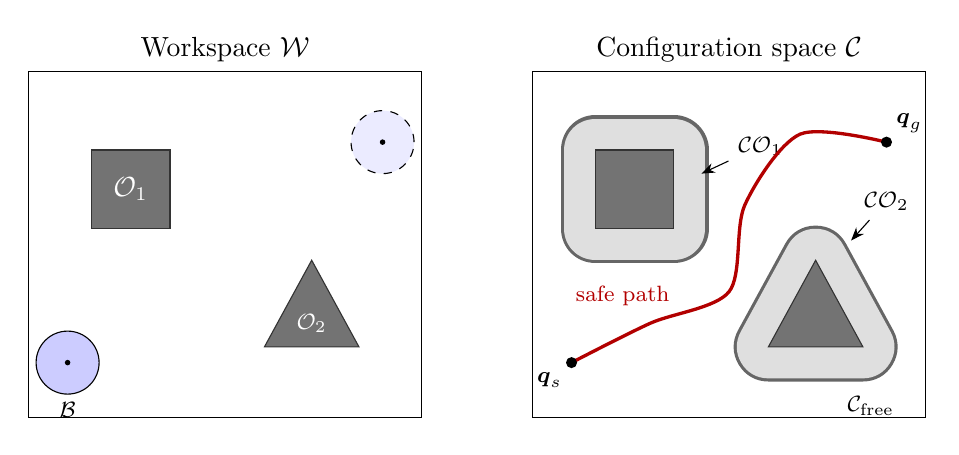
\begin{tikzpicture}[>=Stealth]
\tikzset{obs/.style={fill=black!55,draw=black!80}}
% ---------------- workspace ----------------
\begin{scope}
  \draw (0,0) rectangle (5,4.4);
  \node[above] at (2.5,4.4) {Workspace $\Wspace$};
  \fill[obs] (0.8,2.4) rectangle (1.8,3.4);
  \node[white] at (1.3,2.9) {$\Obs_1$};
  \fill[obs] (3.0,0.9) -- (4.2,0.9) -- (3.6,2.0) -- cycle;
  \node[white,font=\footnotesize] at (3.6,1.2) {$\Obs_2$};
  \draw[fill=blue!20] (0.5,0.7) circle (0.4);
  \fill (0.5,0.7) circle (1pt);
  \draw[dashed,fill=blue!8] (4.5,3.5) circle (0.4);
  \fill (4.5,3.5) circle (1pt);
  \node[font=\footnotesize] at (0.5,0.1) {$\Rob$};
\end{scope}
% ---------------- configuration space ----------------
\begin{scope}[xshift=6.4cm]
  \draw (0,0) rectangle (5,4.4);
  \node[above] at (2.5,4.4) {Configuration space $\Cspace$};
  % CO1 : obstacle grown by 0.4cm (stroke of width 2r reproduces the Minkowski sum)
  \draw[line width=8.8mm,line join=round,draw=black!60,fill=black!60] (0.8,2.4) rectangle (1.8,3.4);
  \draw[line width=8mm,line join=round,draw=gray!25,fill=gray!25] (0.8,2.4) rectangle (1.8,3.4);
  \draw[line width=8.8mm,line join=round,draw=black!60,fill=black!60] (3.0,0.9) -- (4.2,0.9) -- (3.6,2.0) -- cycle;
  \draw[line width=8mm,line join=round,draw=gray!25,fill=gray!25] (3.0,0.9) -- (4.2,0.9) -- (3.6,2.0) -- cycle;
  \fill[obs] (0.8,2.4) rectangle (1.8,3.4);
  \fill[obs] (3.0,0.9) -- (4.2,0.9) -- (3.6,2.0) -- cycle;
  \node[font=\footnotesize] (c1) at (2.9,3.45) {$\CO_1$};
  \draw[->,thin] (c1) -- (2.15,3.1);
  \node[font=\footnotesize] (c2) at (4.5,2.75) {$\CO_2$};
  \draw[->,thin] (c2) -- (4.05,2.25);
  \node[font=\footnotesize] at (4.3,0.15) {$\Cfree$};
  \draw[red!70!black,very thick] plot[smooth] coordinates {(0.5,0.7) (1.5,1.2) (2.5,1.6) (2.7,2.7) (3.4,3.6) (4.5,3.5)};
  \fill (0.5,0.7) circle (2pt) node[below left,font=\footnotesize] {$\qs$};
  \fill (4.5,3.5) circle (2pt) node[above right,font=\footnotesize] {$\qg$};
  \node[red!70!black,font=\footnotesize] at (1.15,1.55) {safe path};
\end{scope}
\end{tikzpicture}
\caption{A disk robot translating in the plane. Left: workspace with two obstacles and the robot at start and goal. Right: in $\Cspace$ the robot is a point and each obstacle is inflated by the robot radius; a safe path stays in $\Cfree$.}
\label{fig:canonical}
\end{figure}

\begin{proposition}[Solvability]
\label{prop:solvability}
The canonical problem admits a solution if and only if $\qs$ and $\qg$ belong to the same connected component of $\Cfree$.
\end{proposition}
\begin{proof}
A safe path from $\qs$ to $\qg$ is, by definition, a continuous curve contained in $\Cfree$ with those end points. Such a curve exists exactly when the two points can be joined inside $\Cfree$, i.e.\ when they lie in the same (path-)connected component of $\Cfree$.
\end{proof}

\begin{remark}
$\CO$ in general consists of several \emph{unconnected} regions, and $\Cfree$ may be disconnected. A planner must therefore return a safe path when $\qs,\qg$ are in the same connected component of $\Cfree$ and a \emph{failure} otherwise.
\end{remark}

\begin{intuition}
Think of $\Cfree$ as a map of ``islands'': you can walk from $\qs$ to $\qg$ without getting your feet wet only if they are on the same island. Reporting a failure is not giving up: it is a \emph{correct answer} when they are not.
\end{intuition}

\subsect{\texorpdfstring{$\Cspace$}{C}-obstacles for single-body robots}{7--9}

Shape and size of $\CO_i$ depend on three things: the obstacle shape, the robot shape, and the robot's movement capabilities (translation only, or also rotation).

\paragraph{Robot that only translates.}
Let $\Rob_0$ denote the region occupied by the robot when its representative point is at the origin, so that $\Rob(\vq)=\vq+\Rob_0$.

\begin{proposition}[$\Cspace$-obstacle of a translating robot]
\label{prop:mink}
If the robot only translates (fixed orientation), $\Cspace$ is a copy of $\Wspace$ and
\[
  \CO_i=\Obs_i\Mink(-\Rob_0)=\{\,o-b:\ o\in\Obs_i,\ b\in\Rob_0\,\}.
\]
\end{proposition}
\begin{proof}
$\vq\in\CO_i$ iff $(\vq+\Rob_0)\cap\Obs_i\neq\emptyset$ iff there exist $b\in\Rob_0$ and $o\in\Obs_i$ with $\vq+b=o$, i.e.\ $\vq=o-b$.
\end{proof}

\begin{intuition}
Slide the robot around the obstacle, keeping it in contact but never overlapping, and record the trajectory of its representative point: that closed curve is the boundary of $\CO_i$. The ``$-\Rob_0$'' is the robot flipped through its representative point: if the robot sticks out to the right of the point, the obstacle has to be inflated on the \emph{left}.
\end{intuition}

\begin{example}[Point robot]
$\Rob_0=\{\mathbf 0\}$, hence $\CO_i=\Obs_i$: $\Cspace$ is a copy of $\Wspace$ and $\Cspace$-obstacles are copies of the obstacles.
\end{example}

\begin{example}[Disk robot, translation only]
$\Rob_0$ is a disk of radius $r$ centred at the origin, which is symmetric ($-\Rob_0=\Rob_0$), and $\vq$ are the Cartesian coordinates of the centre. Then $\CO_i=\Obs_i\Mink\Rob_0$ is the obstacle \emph{grown isotropically} by $r$ in every direction. If $\Obs_i$ is a polygon, $\CO_i$ is a \emph{generalized polygon}: its boundary consists of line segments (parallel to the original edges at distance $r$) and circular arcs of radius $r$ around the vertices. Figure~\ref{fig:canonical} shows this for a rectangle and a triangle.
\end{example}

\begin{example}[Polygonal robot, translation only]
\label{ex:poly}
Let the obstacle be the rectangle $[1,3]\times[1,2.5]$ and let the robot be the right triangle with vertices $(0,0),(1,0),(0,0.8)$ relative to its representative vertex $\boldsymbol p$ (the right-angle vertex). Then $-\Rob_0$ has vertices $(0,0),(-1,0),(0,-0.8)$, and the convex hull of the rectangle's four corners shifted by each of them gives the pentagon with vertices
\[
  (0,1),\ (1,0.2),\ (3,0.2),\ (3,2.5),\ (0,2.5).
\]
It is a polygon (no arcs), and it is grown \emph{anisotropically}: by $1$ on the left, by $0.8$ at the bottom, and not at all to the right or at the top. Two placements of the robot touching the obstacle are marked in Fig.~\ref{fig:poly}.
\end{example}

\begin{figure}[H]
\centering
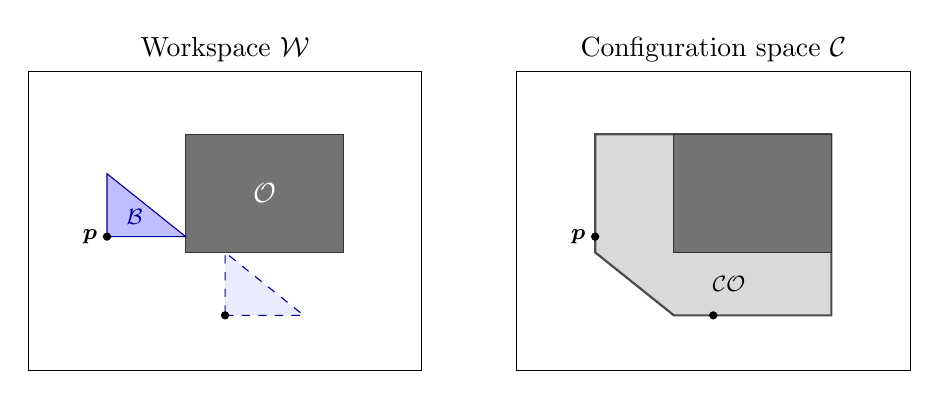
\begin{tikzpicture}[>=Stealth]
\tikzset{obs/.style={fill=black!55,draw=black!80}}
\begin{scope}
  \draw (-1,-0.5) rectangle (4,3.3);
  \node[above] at (1.5,3.3) {Workspace $\Wspace$};
  \fill[obs] (1,1) rectangle (3,2.5);
  \node[white] at (2,1.75) {$\Obs$};
  \fill[blue!25,draw=blue!60!black] (0,1.2) -- (1,1.2) -- (0,2.0) -- cycle;
  \fill (0,1.2) circle (1.5pt) node[left,font=\footnotesize] {$\boldsymbol p$};
  \draw[dashed,blue!60!black,fill=blue!8] (1.5,0.2) -- (2.5,0.2) -- (1.5,1.0) -- cycle;
  \fill (1.5,0.2) circle (1.5pt);
  \node[font=\footnotesize,blue!60!black] at (0.35,1.45) {$\Rob$};
\end{scope}
\begin{scope}[xshift=6.2cm]
  \draw (-1,-0.5) rectangle (4,3.3);
  \node[above] at (1.5,3.3) {Configuration space $\Cspace$};
  \fill[gray!30,draw=black!70,thick] (0,1) -- (1,0.2) -- (3,0.2) -- (3,2.5) -- (0,2.5) -- cycle;
  \fill[obs] (1,1) rectangle (3,2.5);
  \node[font=\footnotesize] at (1.7,0.6) {$\CO$};
  \fill (0,1.2) circle (1.5pt) node[left,font=\footnotesize] {$\boldsymbol p$};
  \fill (1.5,0.2) circle (1.5pt);
  \node[font=\footnotesize,anchor=north] at (1.5,0.1) {};
\end{scope}
\end{tikzpicture}
\caption{Example~\ref{ex:poly}: a triangular robot translating around a rectangular obstacle. In $\Cspace$ the representative vertex $\boldsymbol p$ moves along the boundary of the pentagon $\CO=\Obs\Mink(-\Rob_0)$, which is larger than $\Obs$ and grown anisotropically.}
\label{fig:poly}
\end{figure}

\begin{remark}
The \emph{position} of $\CO_i$ depends on which point of the robot is chosen as representative ($\vq$): changing it translates $\Rob_0$, and therefore translates $\CO_i$ rigidly, with the same shape. What matters is that $\vq$ and $\CO_i$ are defined consistently. For convex polygons with $n_O$ and $n_B$ vertices the Minkowski sum has at most $n_O+n_B$ vertices.
\end{remark}

\paragraph{Robot that translates and rotates.}
Now $\vq=(x,y,\theta)$ and $\Rob(\vq)=\boldsymbol p+R(\theta)\Rob_0$. The configuration space contains an angle, hence it is a manifold ($\R^2\times S^1$), but for drawing purposes it is represented naively as $\R^3$. For each fixed orientation $\theta$ the slice is again a Minkowski sum:
\[
  \CO_i(\theta)=\Obs_i\Mink\bigl(-R(\theta)\Rob_0\bigr),\qquad
  \CO_i=\bigcup_{\theta}\ \CO_i(\theta)\times\{\theta\}.
\]
Hence $\CO_i$ is obtained from the original obstacle via a \emph{grow and stack} procedure: draw the planar $\CO_i$ for each value of $\theta$ in the $(x,y)$ plane and stack all slices along the $\theta$ axis.

\begin{figure}[H]
	\centering
	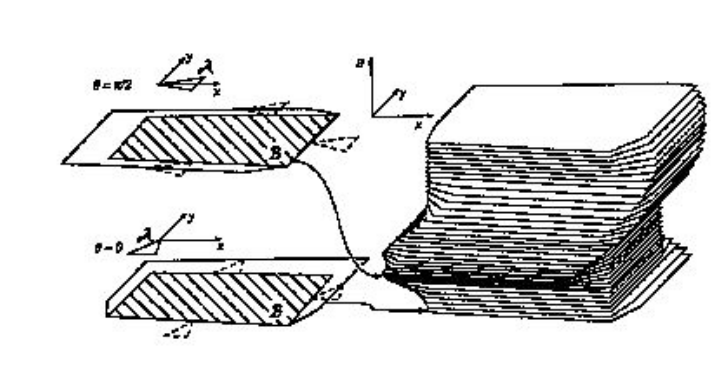
\includegraphics[width=1.0\linewidth]{1795433270836.png}
	\caption{Grow-and-stack construction of the $\Cspace$-obstacle for a polygonal robot that translates and rotates.}\label{fig:stack}
\end{figure}

\begin{intuition}
Rotating the robot changes its footprint, so every orientation gives a different ``inflated obstacle''; the real $\Cspace$-obstacle is the pile of all these slices, a twisted three-dimensional solid. Already for one rigid body in the plane the construction is heavy; for multi-body robots it quickly becomes impractical.
\end{intuition}

\subsect{\texorpdfstring{$\Cspace$}{C}-obstacles for manipulators}{10--12}

For a fixed-base manipulator $\Rob$ made of rigid links $\Rob_1,\dots,\Rob_n$ there are \emph{two} kinds of $\Cspace$-obstacles, arising from
\begin{itemize}
  \item collisions between a link $\Rob_i$ and an obstacle $\Obs_j$;
  \item \emph{self-collisions}, i.e.\ interference between two links $\Rob_i$ and $\Rob_j$ of the manipulator.
\end{itemize}
Even considering only the first kind, building $\Cspace$-obstacles is much more complicated than for single-body robots: computing the boundary of $\CO_i$ requires \emph{inverse kinematics} to identify all the configurations that bring one or more links in contact with $\Obs_i$.

The two 2R planar manipulator scenes of the slides make two points that are typical in $\Cspace$ (here $\Cspace$ is a torus, drawn as the square $[0,2\pi]^2$ with opposite sides identified):

\begin{itemize}
  \item \textbf{Scene 1:} disjoint workspace obstacles may \emph{merge} in $\Cspace$ (the two obstacles of $\Wspace$ give rise to connected, elongated, curved $\Cspace$-obstacles);
  \item \textbf{Scene 2:} $\Cfree$ may be \emph{disconnected}: with several obstacles, some regions of configurations are separated from each other and, to move from one to the other, a collision would be necessary.
\end{itemize}


\begin{figure}[H]
	\centering
	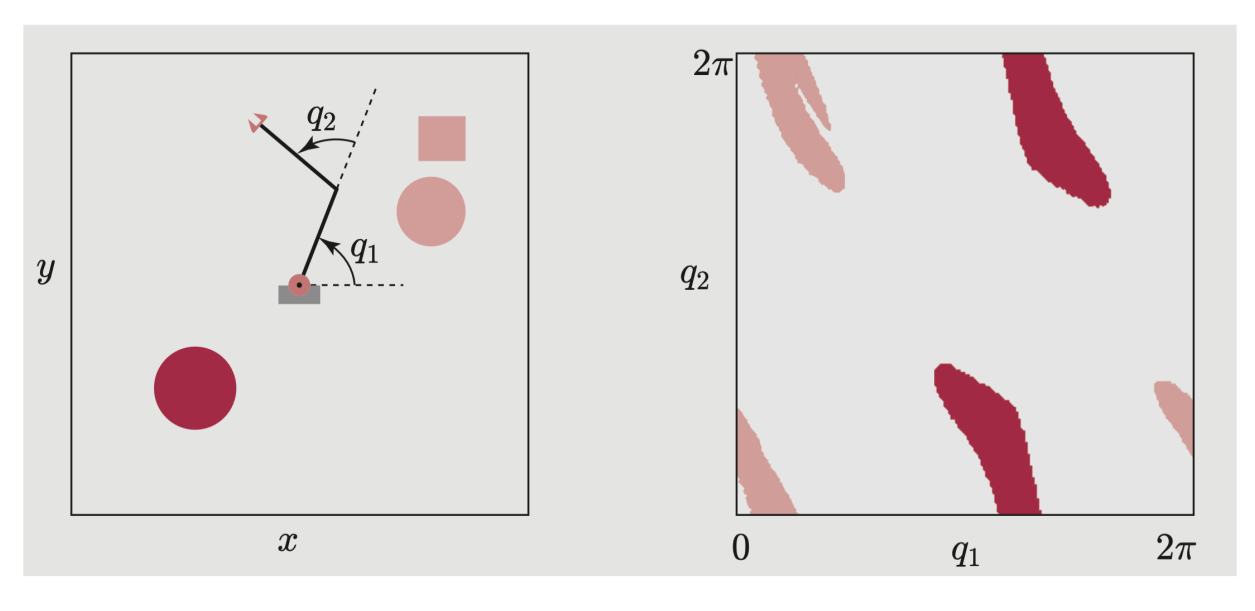
\includegraphics[width=1.0\linewidth]{1795433331699.png}
	\caption{Two scenes for a 2R manipulator and their $\Cspace$-obstacles.}\label{fig:2R}
\end{figure}
\begin{intuition}
Obstacles that are far apart in the workspace can be adjacent in $\Cspace$: what matters is not where the obstacles are, but which \emph{poses of the whole arm} they forbid. A very simple workspace (a few discs and polygons) can already produce a tangled, disconnected $\Cfree$, which is why the geometry of $\Cspace$ cannot be guessed from the workspace by eye.
\end{intuition}

% =====================================================================
\sect{Motion Planning Methods}{13--14}
% =====================================================================

All motion planning methods work, in principle, in the configuration space $\Cspace$. Many of them (but not all) need a preliminary computation of the $\Cspace$-obstacle region $\CO$.

\paragraph{Computing $\CO$.} It is a highly expensive procedure, whose complexity is exponential in $\dim\Cspace$. There are two approaches:
\begin{itemize}
  \item \textbf{exact}: it requires an algebraic model of $\Obs_1,\dots,\Obs_p$ (the examples above belong here);
  \item \textbf{approximate}: sample $\Cspace$ with a regular grid, compute the volume occupied by the robot at each sample, and check for collisions between this volume and the obstacles. Typically only a single point per grid cell (e.g.\ its centre) is tested: if its configuration $(x_c,y_c,\theta_c)$ leads to a collision the cell is marked \emph{occupied}, otherwise \emph{free}.
\end{itemize}

Checking whether a \emph{single} configuration is in collision is relatively fast, and efficient collision-checking algorithms exist (for a 7-dof arm, less than $1$\,ms on a CPU). The approximate approach is therefore a ``brute-force'' loop of cheap tests.

\begin{intuition}
Describing the shape of $\CO$ analytically is like writing down an equation for the coastline of a country; asking ``is this particular point in the sea?'' is trivial. Because the \emph{point query} is cheap and the \emph{global description} is expensive, a whole family of methods (probabilistic and potential-field methods) avoid $\CO$ and use only the point query.
\end{intuition}

\subsect{Classification}{14}

\begin{definition}[Classes of motion planning methods]
Motion planning methods fall into three classes.
\begin{enumerate}
  \item \textbf{Roadmap methods} (need $\CO$): represent the connectivity of $\Cfree$ by a sufficiently rich network of safe paths (a \emph{roadmap}); e.g.\ retraction, cell decomposition.
  \item \textbf{Probabilistic methods} (do not need $\CO$): a particular instance of sampling-based methods in which samples of $\Cspace$ are randomly extracted; e.g.\ PRM, RRT.
  \item \textbf{Artificial potential field methods} (do not need $\CO$): a heuristic approach particularly suitable for on-line planning.
\end{enumerate}
\end{definition}

\begin{definition}[Roadmap]
A \emph{roadmap} is a network (graph) of safe paths contained in $\Cfree$ such that (i) any configuration of $\Cfree$ can be easily connected to it by a safe path, and (ii) it preserves the connectivity of $\Cfree$: two points lie in the same connected component of $\Cfree$ iff they connect to the same connected component of the roadmap.
\end{definition}

Planning then reduces to (a) connecting $\qs$ and $\qg$ to the roadmap and (b) searching the graph. We now study two ways of building roadmaps: the retraction method (Sec.~\ref{sec:retraction}) and cell decomposition (Sec.~\ref{sec:cells}).

\begin{intuition}
A roadmap is the ``subway map'' of $\Cfree$: you do not need to know every street, only how to reach a station from where you are and how stations are linked. Once the map exists, a query is a short trip: walk to a station, ride the network, walk from the last station to the goal.
\end{intuition}

% =====================================================================
\sect{Roadmap Method: Retraction}{15--21}
\label{sec:retraction}
% =====================================================================

\subsect{Assumptions and basic definitions}{15}

\begin{definition}[Polygonal limited subset]
In addition to the assumptions of the canonical problem, the retraction method assumes $\Cspace=\R^2$ and that $\Cfree$ is a \emph{polygonal limited subset}: a bounded set whose boundary $\partial\Cfree=\partial\CO$ is entirely made of line segments (it may contain polygonal holes).
\end{definition}

If the obstacles are not polygonal they can be approximated by polygons (for instance, a circular obstacle by a polygon that contains it, which is a conservative approximation).

\begin{definition}[Clearance]
The \emph{clearance} of a configuration $\vq\in\Cfree$ is the minimum distance between $\vq$ and the boundary of $\Cfree$:
\[
  \gamma(\vq)=\min_{\vq'\in\partial\CO}\|\vq-\vq'\|,
\]
where $\|\cdot\|$ denotes an appropriate distance in $\Cspace$.
\end{definition}

\begin{definition}[Neighbors]
The \emph{neighbors} of $\vq\in\Cfree$ are the boundary points that realize its clearance:
\[
  N(\vq)=\{\vq'\in\partial\CO:\ \|\vq-\vq'\|=\gamma(\vq)\}.
\]
\end{definition}

\begin{definition}[Generalized Voronoi diagram]
The \emph{generalized Voronoi diagram} (GVD) of $\Cfree$ is the set of configurations with more than one neighbor:
\[
  \Vor(\Cfree)=\{\vq\in\Cfree:\ \card(N(\vq))>1\}.
\]
\end{definition}

It is called \emph{generalized} because ordinary Voronoi diagrams have \emph{single points} as generators (and each generator owns the region of the plane closer to it than to any other), whereas here the ``generators'' are the polygons (the pieces of $\partial\CO$).

\begin{intuition}
Imagine $\gamma$ as the altitude of a landscape: it is zero on the obstacle boundaries and grows as you move away from them. The GVD is the system of \emph{ridges} of this landscape, the places where two (or more) different obstacle features are exactly equally close. Walking along a ridge means ``walking in the middle of the corridor'', i.e.\ as far from the obstacles as you can be.
\end{intuition}

\subsect{The Voronoi diagram as a roadmap}{16--17}

\begin{proposition}[Elementary arcs of the GVD]
\label{prop:arcs}
The arcs of $\Vor(\Cfree)$ are of three kinds, according to the pair of boundary features that generate them:
\begin{itemize}
  \item \textbf{edge--edge}: a \emph{rectilinear} segment (a piece of the bisector of the two edges);
  \item \textbf{vertex--vertex}: a \emph{rectilinear} segment (a piece of the perpendicular bisector of the two vertices);
  \item \textbf{edge--vertex}: a \emph{parabolic} arc (with the vertex as focus and the line of the edge as directrix).
\end{itemize}
\end{proposition}
\begin{proof}
The points equidistant from two lines lie on their angle bisector; from two points, on the perpendicular bisector of the segment joining them; from a point and a line, on a parabola whose focus is the point and whose directrix is the line. In the last case, e.g.\ for the line $y=0$ and the point $(0,2)$: $y^2=x^2+(y-2)^2\iff y=1+x^2/4$.
\end{proof}

\begin{figure}[H]
\centering
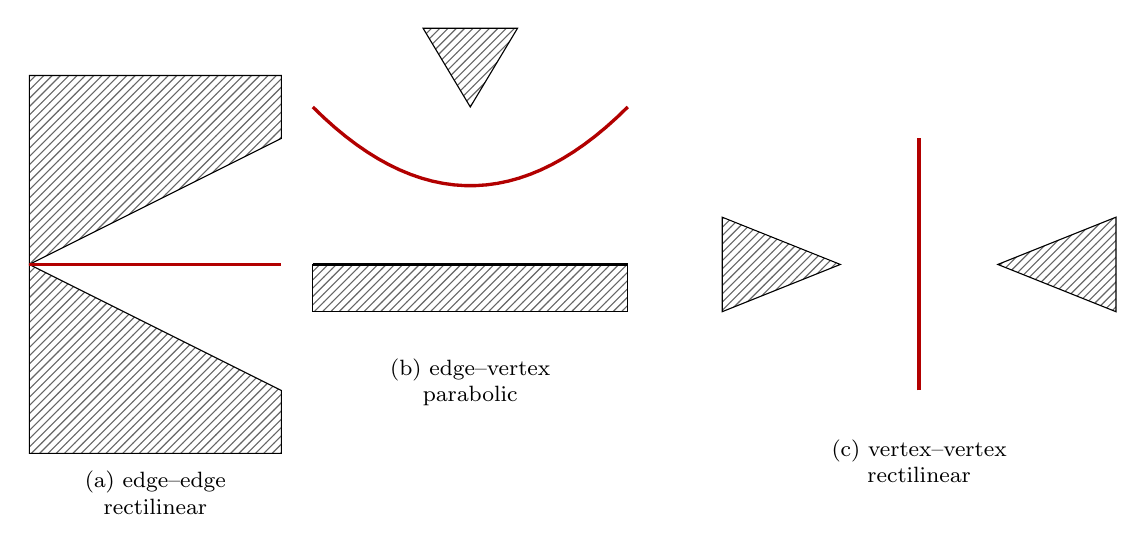
\begin{tikzpicture}[>=Stealth]
\tikzset{wall/.style={pattern=north east lines,pattern color=black!60,draw=black}}
% (a) edge-edge
\begin{scope}
  \fill[wall] (0,0) -- (3.2,1.6) -- (3.2,2.4) -- (0,2.4) -- cycle;
  \fill[wall] (0,0) -- (3.2,-1.6) -- (3.2,-2.4) -- (0,-2.4) -- cycle;
  \draw[red!70!black,very thick] (0,0) -- (3.2,0);
  \node[font=\footnotesize,align=center] at (1.6,-2.9) {(a) edge--edge\\rectilinear};
\end{scope}
% (b) edge-vertex
\begin{scope}[xshift=5.6cm]
  \fill[wall] (-2,0) rectangle (2,-0.6);
  \draw[thick] (-2,0) -- (2,0);
  \fill[wall] (-0.6,3.0) -- (0.6,3.0) -- (0,2.0) -- cycle;
  \draw[red!70!black,very thick,domain=-2:2,samples=30,variable=\t] plot ({\t},{1+\t*\t/4});
  \node[font=\footnotesize,align=center] at (0,-1.5) {(b) edge--vertex\\parabolic};
\end{scope}
% (c) vertex-vertex
\begin{scope}[xshift=11.3cm]
  \fill[wall] (-2.5,-0.6) -- (-2.5,0.6) -- (-1,0) -- cycle;
  \fill[wall] (2.5,-0.6) -- (2.5,0.6) -- (1,0) -- cycle;
  \draw[red!70!black,very thick] (0,-1.6) -- (0,1.6);
  \node[font=\footnotesize,align=center] at (0,-2.5) {(c) vertex--vertex\\rectilinear};
\end{scope}
\end{tikzpicture}
\caption{The three elementary tracts of the GVD (red): points equidistant from two edges, from an edge and a vertex, and from two vertices.}
\label{fig:tracts}
\end{figure}

\begin{intuition}
The three cases are the three ways ``two nearest things'' can look. Between two straight walls the middle is a straight line. Between a straight wall and a pointed corner the middle bends: near the corner the path has to bulge away from it, which is exactly what a parabola does. Between two corners it is the perpendicular bisector.
\end{intuition}

\begin{remark}[GVD as a roadmap]
$\Vor(\Cfree)$ can be seen as a graph whose \emph{arcs} are the elementary arcs of Prop.~\ref{prop:arcs} and whose \emph{nodes} are their end points. It captures the connectivity of $\Cfree$ and it \emph{maximizes safety}, since along its arcs the robot is as far as possible from the two nearest obstacle features: it is a natural roadmap of $\Cfree$.
\end{remark}

\begin{figure}[H]
\centering
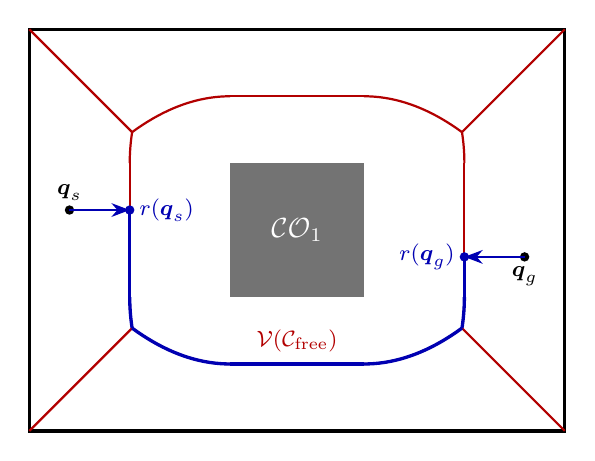
\begin{tikzpicture}[scale=0.85,>=Stealth]
\def\gvdquad{%
  \draw[red!70!black,thick] (0,0) -- (1.536,1.536);
  \draw[red!70!black,thick,domain=1.536:2,samples=12,variable=\t] plot ({1.5+(\t-2)^2/6},{\t});
  \draw[red!70!black,thick] (1.5,2) -- (1.5,3);
  \draw[red!70!black,thick,domain=1.536:3,samples=20,variable=\t] plot ({\t},{1+(\t-3)^2/4});
  \draw[red!70!black,thick] (3,1) -- (4,1);}
\draw[very thick] (0,0) rectangle (8,6);
\fill[black!55] (3,2) rectangle (5,4);
\node[white] at (4,3) {$\CO_1$};
\begin{scope}\gvdquad\end{scope}
\begin{scope}[cm={-1,0,0,1,(8,0)}]\gvdquad\end{scope}
\begin{scope}[cm={1,0,0,-1,(0,6)}]\gvdquad\end{scope}
\begin{scope}[cm={-1,0,0,-1,(8,6)}]\gvdquad\end{scope}
\node[red!70!black,font=\footnotesize] at (4,1.35) {$\Vor(\Cfree)$};
% start/goal and retractions
\fill (0.6,3.3) circle (2pt) node[above,font=\footnotesize] {$\qs$};
\fill (7.4,2.6) circle (2pt) node[below,font=\footnotesize] {$\qg$};
\draw[blue!70!black,thick,->] (0.6,3.3) -- (1.5,3.3);
\draw[blue!70!black,thick,->] (7.4,2.6) -- (6.5,2.6);
\fill[blue!70!black] (1.5,3.3) circle (2pt) node[right,font=\footnotesize] {$r(\qs)$};
\fill[blue!70!black] (6.5,2.6) circle (2pt) node[left,font=\footnotesize] {$r(\qg)$};
% path on V from r(qs) to r(qg) through the lower side
\draw[blue!70!black,very thick] (1.5,3.3) -- (1.5,2);
\draw[blue!70!black,very thick,domain=2:1.536,samples=12,variable=\t] plot ({1.5+(\t-2)^2/6},{\t});
\draw[blue!70!black,very thick,domain=1.536:3,samples=20,variable=\t] plot ({\t},{1+(\t-3)^2/4});
\draw[blue!70!black,very thick] (3,1) -- (5,1);
\draw[blue!70!black,very thick,domain=5:6.464,samples=20,variable=\t] plot ({\t},{1+(\t-5)^2/4});
\draw[blue!70!black,very thick,domain=1.536:2,samples=12,variable=\t] plot ({8-1.5-(\t-2)^2/6},{\t});
\draw[blue!70!black,very thick] (6.5,2) -- (6.5,2.6);
\end{tikzpicture}
\caption{GVD (red) of a rectangular room with a central obstacle: four diagonal branches reach the room corners, and a closed loop surrounds the obstacle, made of straight tracts (edge--edge) and parabolic tracts (edge--vertex around the obstacle corners). The solution path (blue) is $\qs\to r(\qs)$, an arc sequence on $\Vor$, and $r(\qg)\to\qg$.}
\label{fig:gvd}
\end{figure}

\subsect{Retraction}{18}

Usually $\qs$ and $\qg$ do not lie on $\Vor(\Cfree)$, so they must first be connected to the diagram.

\begin{definition}[Retraction]
For $\vq\in\Cfree\setminus\Vor(\Cfree)$ the neighbor $s$ is unique and $\nabla\gamma(\vq)=(\vq-s)/\|\vq-s\|$ is the direction of \emph{clearance growth}. The \emph{retraction} $r(\vq)$ is the first intersection with $\Vor(\Cfree)$ of the ray $r^\circ(\vq)$ that starts at $\vq$ and follows $\nabla\gamma$ (the line through $N(\vq)$ and $\vq$, moving away from $N(\vq)$). For $\vq\in\Vor(\Cfree)$, $r(\vq)=\vq$.
\end{definition}

\begin{proposition}[Retraction preserves connectivity]
\label{prop:retr}
For every $\vq\in\Cfree$, the segment from $\vq$ to $r(\vq)$ is a safe path; in particular $\vq$ and $r(\vq)$ lie in the same connected component of $\Cfree$.
\end{proposition}
\begin{proof}
Let $u=\nabla\gamma(\vq)$ and $s$ the unique neighbor. As long as $s$ remains the \emph{unique} nearest boundary point, the clearance along the ray is $\gamma(\vq+\lambda u)=\gamma(\vq)+\lambda>0$. By definition of $\Vor(\Cfree)$, a second nearest boundary point appears exactly when the ray first meets $\Vor(\Cfree)$, that is, at $r(\vq)$. Hence the clearance stays strictly positive on the whole segment, so the segment never touches $\partial\CO$ and remains in $\Cfree$.
\end{proof}

\begin{intuition}
Retraction means ``walk straight away from the nearest wall until you are equally far from two walls''. Because every step increases the distance from every obstacle point that mattered, you can never run into one. Following the clearance is what makes it safe: jumping instead to the \emph{closest} point of the diagram could cross a thin obstacle and land you in a different connected component, with lower distance but no preserved connectivity.
\end{intuition}

\begin{figure}[H]
\centering
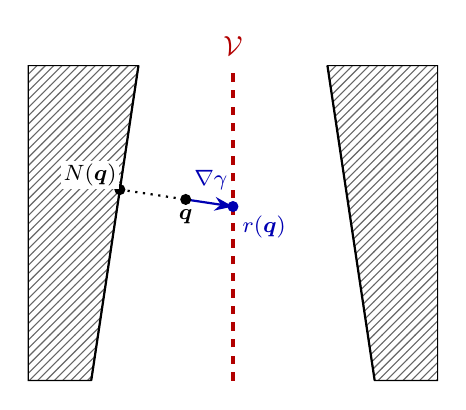
\begin{tikzpicture}[>=Stealth]
\tikzset{wall/.style={pattern=north east lines,pattern color=black!60,draw=black}}
\fill[wall] (-1.8,-1.5) -- (-1.2,2.5) -- (-2.6,2.5) -- (-2.6,-1.5) -- cycle;
\fill[wall] (1.8,-1.5) -- (1.2,2.5) -- (2.6,2.5) -- (2.6,-1.5) -- cycle;
\draw[thick] (-1.8,-1.5) -- (-1.2,2.5);
\draw[thick] (1.8,-1.5) -- (1.2,2.5);
\draw[red!70!black,very thick,dashed] (0,-1.5) -- (0,2.5);
\node[red!70!black,above] at (0,2.5) {$\Vor$};
\coordinate (q) at (-0.6,0.8);
\coordinate (N) at (-1.436,0.925);
\coordinate (r) at (0,0.71);
\draw[dotted,thick] (N) -- (q);
\draw[->,thick,blue!70!black] (q) -- (r);
\fill (q) circle (2pt) node[below,font=\footnotesize] {$\vq$};
\fill (N) circle (2pt) node[above left,font=\footnotesize,fill=white,inner sep=1pt] {$N(\vq)$};
\fill[blue!70!black] (r) circle (2pt) node[below right,font=\footnotesize] {$r(\vq)$};
\node[font=\footnotesize,blue!70!black,above] at (-0.28,0.8) {$\nabla\gamma$};
\end{tikzpicture}
\caption{Retraction of $\vq$ onto the Voronoi diagram between two walls: move along the direction of clearance growth (away from the neighbor $N(\vq)$) until the first point $r(\vq)$ of $\Vor$.}
\label{fig:retraction}
\end{figure}

\begin{theorem}[Existence of a safe path]
\label{thm:retr}
A safe path between $\qs$ and $\qg$ exists if and only if a path exists on $\Vor(\Cfree)$ between $r(\qs)$ and $r(\qg)$.
\end{theorem}
\begin{proof}[Proof sketch]
($\Leftarrow$) Concatenate the safe segments $\qs\to r(\qs)$ and $r(\qg)\to\qg$ (Prop.~\ref{prop:retr}) with the path on $\Vor(\Cfree)\subset\Cfree$.
($\Rightarrow$) Let $K$ be the connected component of $\Cfree$ containing $\qs$ and $\qg$ (Prop.~\ref{prop:solvability}). The map $r$ is continuous and sends $K$ onto $\Vor(\Cfree)\cap K$, so this set is connected, being a continuous image of a connected set. Since $\Vor(\Cfree)$ is a finite graph, a connected subset of it is path-connected; as $r(\qs),r(\qg)\in\Vor(\Cfree)\cap K$, they are joined by a path on $\Vor(\Cfree)$.
\end{proof}

\begin{intuition}
The theorem turns a two-dimensional question (``can I get through this maze of free space?'') into a one-dimensional one (``are these two points on the same piece of this graph?''). The name of the method comes from here: a retraction brings a configuration of the two-dimensional $\Cfree$ down to the one-dimensional set $\Vor(\Cfree)$, without breaking connectivity.
\end{intuition}

\subsect{Algorithm, solution path and properties}{19--21}

\begin{algorithm}[Retraction method]
\label{alg:retr}
The method consists of the following steps.
\begin{enumerate}
  \item Build the generalized Voronoi diagram $\Vor(\Cfree)$.
  \item Compute the retractions $r(\qs)$ and $r(\qg)$.
  \item Search $\Vor(\Cfree)$ for a sequence of arcs such that $r(\qs)$ belongs to the first and $r(\qg)$ to the last.
  \item If the search is successful, return the solution path made of:
  \begin{enumerate}[label=(\alph*)]
    \item the line segment from $\qs$ to $r(\qs)$;
    \item the portion of the first arc from $r(\qs)$ to its end;
    \item the second, third, \dots, penultimate arcs;
    \item the portion of the last arc from its start to $r(\qg)$;
    \item the line segment from $r(\qg)$ to $\qg$.
  \end{enumerate}
  Otherwise, report a failure.
\end{enumerate}
\end{algorithm}

Figure~\ref{fig:gvd} shows a solution path produced by this procedure.

\paragraph{Minimum-length path.} If a minimum-length path is desired, in the graph search of step~3 label each arc with a cost equal to its length and use Dijkstra or $\mathrm{A}^\star$ to compute a minimum-cost solution.

\begin{definition}[Completeness; multiple-query]
A planner is \emph{complete} if it finds a solution whenever one exists and reports a failure otherwise. A planner is \emph{multiple-query} if the data structure it builds depends only on the environment, so that it can be built once and reused for different pairs $(\qs,\qg)$.
\end{definition}

\begin{theorem}[Properties of the retraction method]
\label{thm:retr-props}
The retraction method is (i) complete, (ii) multiple-query, and (iii) if $\Cfree$ has $v$ vertices, $\Vor(\Cfree)$ has $O(v)$ arcs and the overall time complexity is $O(v\log v)$.
\end{theorem}
\begin{proof}[Proof sketch]
(i) follows from Theorem~\ref{thm:retr}: the graph search on a finite graph is exhaustive, so it finds a path iff one exists. (ii) $\Vor(\Cfree)$ depends only on $\Cfree$, hence it can be built once for all; only steps 2--4 depend on $\qs,\qg$. (iii) The cost of the steps is: step~1, $O(v\log v)$; step~2, $O(v)$; step~3, $O(v\log v)$ ($\mathrm{A}^\star$ on a graph with $O(v)$ arcs). The sum is $O(v\log v)$.
\end{proof}

\begin{intuition}
Because the diagram is built once, the expensive part ($O(v\log v)$) is paid at ``preprocessing'' time; later queries only retract two points and search a graph that is linear in the number of vertices. Completeness is the real gift of the method: if it says ``failure'', no path exists.
\end{intuition}

\begin{remark}[Extensions]
Extensions of the retraction method to higher-dimensional configuration spaces, or without the polygonal assumption, are possible but quite complicated and not very efficient.
\end{remark}

% =====================================================================
\sect{Roadmap Method: Cell Decomposition}{22--32}
\label{sec:cells}
% =====================================================================

\subsect{General idea}{22}

\begin{definition}[Cell decomposition and connectivity graph]
A \emph{cell decomposition} of $\Cfree$ is a collection of regions (\emph{cells}) with disjoint interiors that cover $\Cfree$ (exact decomposition) or a part of it (approximate decomposition) and such that
\begin{enumerate}
  \item[(P1)] it is easy to compute a safe path between two configurations in the \emph{same} cell;
  \item[(P2)] it is easy to compute a safe path between two configurations in \emph{adjacent} cells.
\end{enumerate}
The associated \emph{connectivity graph} $\mathcal{C}$ has the cells as nodes and an arc between two nodes iff the cells are adjacent. A path on $\mathcal{C}$ is a sequence of adjacent cells called a \emph{channel}.
\end{definition}

Once a decomposition is available, we find a channel with $\qs$ in the first cell and $\qg$ in the last, and extract a safe path inside it. Different methods are obtained depending on the \emph{type of cells}:
\begin{itemize}
  \item \textbf{exact decomposition}: cells have variable shapes and cover exactly the whole $\Cfree$;
  \item \textbf{approximate decomposition}: for simplicity all cells have the same (fixed) shape, e.g.\ squares, so the decomposition does not cover all of $\Cfree$.
\end{itemize}

\begin{proposition}
\label{prop:channel}
If (P1) and (P2) hold, every channel from the cell containing $\qs$ to the cell containing $\qg$ yields a safe path from $\qs$ to $\qg$.
\end{proposition}
\begin{proof}
Choose a configuration in the common boundary of each pair of consecutive cells of the channel; join $\qs$ to the first, each to the next, and the last to $\qg$. Each leg stays in a single cell (P1) or crosses between adjacent cells (P2); all cells are in $\Cfree$.
\end{proof}

\begin{intuition}
It is the ``rooms and doors'' idea: if you know how to walk inside a room (easy) and how to pass through a door between neighbouring rooms (easy), a route from the start room to the goal room is just a list of rooms, i.e.\ a path on the graph of rooms. A channel is also more than a single path: it is a whole corridor of safe configurations.
\end{intuition}

\subsect{Exact decomposition}{23--28}

\paragraph{Assumptions and cells.} Assume $\Cspace=\R^2$ and $\Cfree$ a polygonal limited subset. Variable-shape cells are needed to decompose $\Cfree$ exactly; a typical choice are \emph{convex polygons}.

\begin{lemma}[Convex cells satisfy (P1) and (P2)]
\label{lem:convex}
Let $c_1,c_2$ be convex polygonal cells sharing a boundary segment $\Gamma$ with midpoint $m$. Then any two points of $c_1$ are joined by a straight segment contained in $c_1$ (P1), and for $\boldsymbol p\in c_1$, $\boldsymbol p'\in c_2$ the polyline $\boldsymbol p\to m\to\boldsymbol p'$ is contained in $c_1\cup c_2$ (P2).
\end{lemma}
\begin{proof}
A convex set contains the segment between any two of its points, which gives (P1). For (P2), $m\in c_1\cap c_2$, so the segment $\boldsymbol p m$ lies in $c_1$ and the segment $m\boldsymbol p'$ lies in $c_2$.
\end{proof}

\begin{intuition}
Convexity means ``no corners to hide behind'': any two points in the cell see each other directly. That is why the decomposition uses convex polygons, and why one never has to search \emph{inside} a cell.
\end{intuition}

\paragraph{Sweep-line algorithm.} It computes a decomposition of $\Cfree$ into convex polygons:
\begin{itemize}
  \item sweep a (vertical) line over $\Cfree$; when it goes through a vertex, two segments, the \emph{extensions}, originate at the vertex (one upward, one downward);
  \item an extension lying in $\Cfree$ is part of the boundary of a cell; the others are discarded (they run inside an obstacle);
  \item the cells are bounded by extensions and/or parts of $\partial\Cfree$; the result is a \emph{trapezoidal decomposition}.
\end{itemize}

\begin{proposition}[Trapezoidal decomposition]
\label{prop:trap}
The sweep-line algorithm decomposes a polygonal limited $\Cfree$ with $v$ vertices into $O(v)$ convex cells (trapezoids, possibly degenerate into triangles).
\end{proposition}
\begin{proof}[Proof sketch]
Each cell is delimited on the left and right by vertical segments (extensions) and above and below by edges of the polygon: it is the intersection of half-planes, hence convex. For the count, the subdivision is a planar graph whose vertices are the $v$ polygon vertices plus at most $2$ end points for each of the at most $2v$ extensions, i.e.\ $O(v)$ vertices; by Euler's formula a planar graph with $O(v)$ vertices has $O(v)$ edges and faces.
\end{proof}

\begin{figure}[H]
\centering
	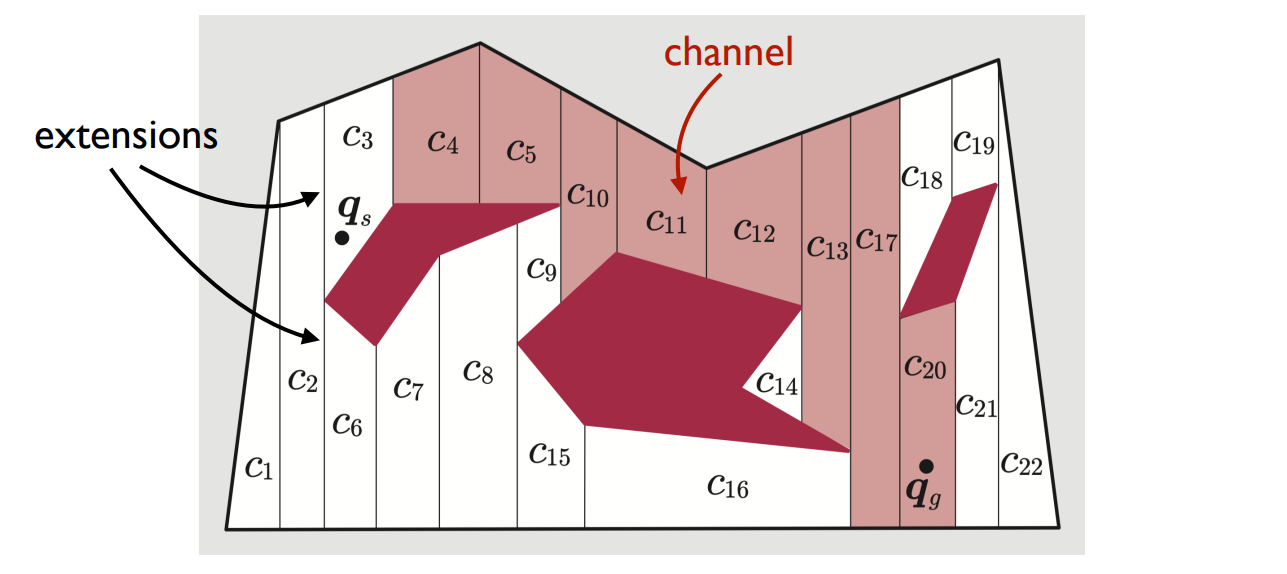
\includegraphics[width=.4\linewidth]{1795681352043.png}
% connectivity graph
	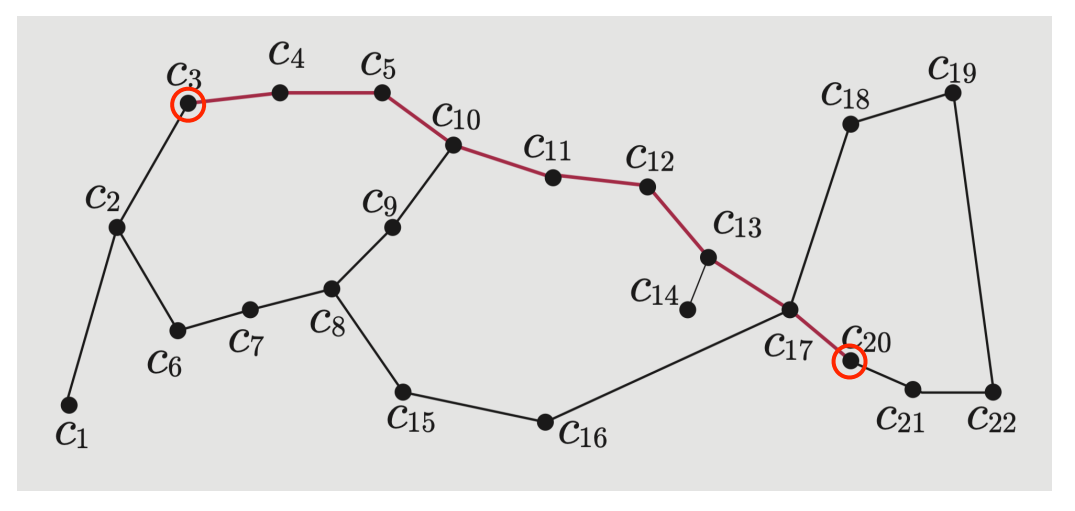
\includegraphics[width=.4\linewidth]{1795681398629.png}
\caption{Sweep-line (trapezoidal) decomposition of a polygonal $\Cfree$ with different obstacles: vertical extensions (dashed) from the vertices cut $\Cfree$ into convex cells. The channel (red in the graph) gives the solution path through the midpoints of the common boundaries.}
\label{fig:trap}
\end{figure}

\paragraph{Algorithm.} After the decomposition we build the connectivity graph $\mathcal{C}$ (nodes: cells; arcs: adjacency), identify the nodes $c_s,c_g$ containing $\qs,\qg$, and use graph search on $\mathcal{C}$ to find a channel from $c_s$ to $c_g$. From the channel, a safe solution path is extracted by joining $\qs$ to $\qg$ via the \emph{midpoints} of the common boundaries (Lemma~\ref{lem:convex}).

\begin{algorithm}[Exact cell decomposition]
\label{alg:exact}
The method consists of the following steps.
\begin{enumerate}
  \item Compute a convex polygonal decomposition of $\Cfree$.
  \item Build the associated connectivity graph $\mathcal{C}$.
  \item Search $\mathcal{C}$ for a channel of cells from $c_s$ to $c_g$.
  \item If successful, extract and return a solution path consisting of
  \begin{enumerate}[label=(\alph*)]
    \item a line segment from $\qs$ to the midpoint of the common boundary between the first two cells;
    \item line segments between the midpoints of consecutive cells;
    \item a line segment from the midpoint of the common boundary between the last two cells to $\qg$.
  \end{enumerate}
  Otherwise, report a failure.
\end{enumerate}
\end{algorithm}

\paragraph{Minimum-length channel.} If a minimum-length path is desired, define a modified connectivity graph with $\qs$, $\qg$ and \emph{all the midpoints} as nodes and with line segments between nodes in the same cell as arcs, each with cost equal to its length, and use $\mathrm{A}^\star$ to compute a minimum-cost path.

\begin{theorem}[Properties of exact cell decomposition]
\label{thm:exact-props}
The exact cell decomposition method is complete and multiple-query. If $\Cfree$ has $v$ vertices, $\mathcal{C}$ has $O(v)$ arcs and the overall complexity is $O(v\log v)$: step~1 costs $O(v\log v)$, step~2 costs $O(v)$ and step~3 costs $O(v\log v)$ ($\mathrm{A}^\star$ on a graph with $O(v)$ arcs).
\end{theorem}
\begin{proof}[Proof sketch]
Completeness: the cells cover $\Cfree$ exactly and adjacency is exact, so a safe path exists iff the connectivity graph has a path between $c_s$ and $c_g$ (Prop.~\ref{prop:channel} for one direction; for the other, a safe path crosses a sequence of cells that is a path on $\mathcal{C}$). The decomposition depends only on $\Cfree$, hence it is multiple-query. The bounds follow from Prop.~\ref{prop:trap}.
\end{proof}

\begin{intuition}
Retraction and exact decomposition behave very similarly (same completeness, same $O(v\log v)$), but the output is different: a roadmap gives \emph{one} curve per query, while a channel contains an \emph{infinity} of safe paths. That extra freedom can be spent to account for nonholonomic constraints or to avoid unexpected obstacles during the motion.
\end{intuition}

\begin{remark}[Comparison and extensions]
\leavevmode
\begin{itemize}
  \item The solution path is a broken line, but smoothing may be performed as a post-processing phase, as long as the path stays within the channel.
  \item An extension to configuration spaces of arbitrary dimension exists, but it is very inefficient: the complexity is exponential in $\dim\Cspace$.
  \item If $\Cspace=\R^3$ and $\Cfree$ is a polyhedral limited subset, the \emph{sweep-plane} algorithm may be used to decompose $\Cfree$ into convex polyhedra.
\end{itemize}
\end{remark}

\subsect{Approximate decomposition}{29--32}

Assume again $\Cspace=\R^2$ and $\Cfree$ a polygonal limited subset. Fixed-shape cells (e.g.\ squares) are used to obtain an approximate decomposition \emph{by defect} of $\Cfree$ (the cells are inside $\Cfree$); convexity still guarantees (P1) and (P2). A \emph{recursive} algorithm reaches a trade-off between simplicity and accuracy: it refines the decomposition only where needed.

\begin{definition}[Cell classification]
A cell is
\begin{itemize}
  \item \emph{free}, if its interior is completely in $\Cfree$;
  \item \emph{occupied}, if it is completely in $\CO$;
  \item \emph{mixed}, if it is neither free nor occupied.
\end{itemize}
\end{definition}

\begin{algorithm}[Recursive approximate cell decomposition]
\label{alg:approx}
Start by dividing $\Cspace$ into $4$ cells and classifying each of them. Then repeat:
\begin{enumerate}
  \item build the connectivity graph $\mathcal{C}$ associated to the current level of decomposition, with \emph{free and mixed} cells as nodes and arcs between adjacent nodes;
  \item identify the nodes $c_s,c_g$ where $\qs,\qg$ are, and use graph search to look for a path (channel) on $\mathcal{C}$ from $c_s$ to $c_g$; if it does not exist, report a failure;
  \item if a channel exists, take any mixed cell in it and decompose it (into $4$ cells) as before.
\end{enumerate}
Stop when a path made \emph{only of free cells} is found, or when a minimum size has been reached for the cells; in the latter case, backtrack.
\end{algorithm}

\begin{figure}[H]
\centering
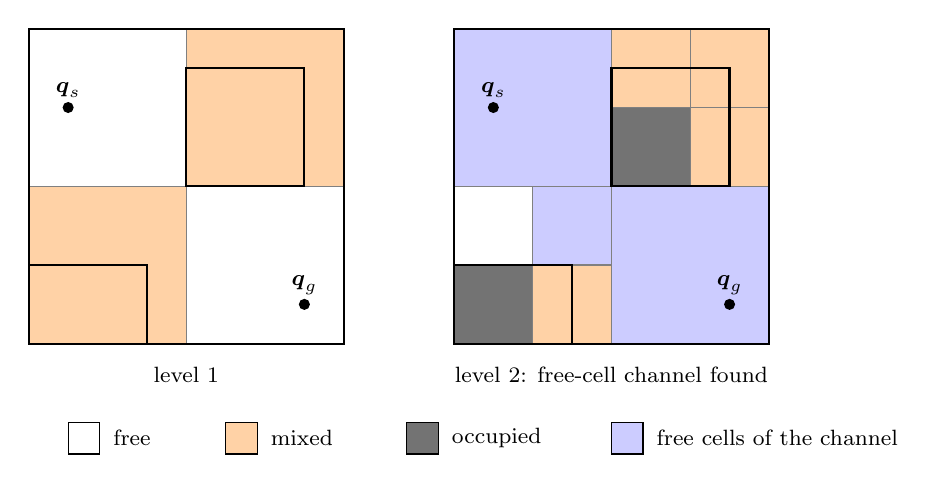
\begin{tikzpicture}[>=Stealth]
\tikzset{occ/.style={fill=black!55},mix/.style={fill=orange!35},chan/.style={fill=blue!20}}
\newcommand{\cell}[4]{\fill[#4] (#1,#2) rectangle ++(#3,#3);}
% ---- level 1 ----
\begin{scope}
  \cell{0}{0}{2}{mix}  \cell{2}{2}{2}{mix}
  \draw[gray] (0,0) grid[step=2] (4,4);
  \draw[thick] (0,0) rectangle (4,4);
  \draw[thick,black] (2,2) rectangle (3.5,3.5);
  \draw[thick,black] (0,0) rectangle (1.5,1);
  \fill (0.5,3) circle (2pt) node[above,font=\footnotesize] {$\qs$};
  \fill (3.5,0.5) circle (2pt) node[above,font=\footnotesize] {$\qg$};
  \node[font=\footnotesize] at (2,-0.4) {level 1};
\end{scope}
% ---- level 2 ----
\begin{scope}[xshift=5.4cm]
  \cell{0}{2}{2}{chan} \cell{2}{0}{2}{chan} \cell{1}{1}{1}{chan}
  \cell{0}{0}{1}{occ} \cell{1}{0}{1}{mix}
  \cell{2}{2}{1}{occ} \cell{3}{2}{1}{mix} \cell{2}{3}{1}{mix} \cell{3}{3}{1}{mix}
  \draw[gray] (0,0) grid[step=2] (4,4);
  \draw[gray] (0,0) grid[step=1] (2,2);
  \draw[gray] (2,2) grid[step=1] (4,4);
  \draw[thick] (0,0) rectangle (4,4);
  \draw[thick,black] (2,2) rectangle (3.5,3.5);
  \draw[thick,black] (0,0) rectangle (1.5,1);
  \fill (0.5,3) circle (2pt) node[above,font=\footnotesize] {$\qs$};
  \fill (3.5,0.5) circle (2pt) node[above,font=\footnotesize] {$\qg$};
  \node[font=\footnotesize] at (2,-0.4) {level 2: free-cell channel found};
\end{scope}
% legend
\begin{scope}[yshift=-1.4cm]
  \fill[white,draw=black] (0.5,0) rectangle (0.9,0.4); \node[right,font=\footnotesize] at (0.95,0.2) {free};
  \fill[orange!35,draw=black] (2.5,0) rectangle (2.9,0.4); \node[right,font=\footnotesize] at (2.95,0.2) {mixed};
  \fill[black!55,draw=black] (4.8,0) rectangle (5.2,0.4); \node[right,font=\footnotesize] at (5.25,0.2) {occupied};
  \fill[blue!20,draw=black] (7.4,0) rectangle (7.8,0.4); \node[right,font=\footnotesize] at (7.85,0.2) {free cells of the channel};
\end{scope}
\end{tikzpicture}
\caption{Recursive decomposition on a $4\times4$ environment with two rectangular obstacles (thick outlines). At level~1 every channel contains a mixed cell; after splitting the mixed cells, a channel made only of free cells (blue) connects the cells containing $\qs$ and $\qg$.}
\label{fig:approx}
\end{figure}

\begin{definition}[Resolution completeness; single-query]
A planner is \emph{resolution complete} if a solution is found if and only if one exists at the maximum allowed resolution (the minimum cell size). It is \emph{single-query} when the data structure depends on the given $\qs,\qg$ (here: the decomposition is guided by them).
\end{definition}

\begin{theorem}[Properties of approximate decomposition]
\label{thm:approx-props}
The recursive approximate cell decomposition is resolution complete and single-query. Recursive decomposition can be implemented efficiently with \emph{quadtrees} (trees whose internal nodes have exactly four children). The method is conceptually applicable to configuration spaces of arbitrary dimension, but its complexity is still exponential in $\dim\Cspace$.
\end{theorem}
\begin{proof}[Proof sketch]
Free cells lie entirely in $\Cfree$, so a channel of free cells always gives a safe path; if the search reports a failure on a graph containing all free \emph{and} mixed cells, no path exists at any finer resolution either, because mixed cells already over-approximate what is traversable. If instead only mixed cells remain at the minimum size, the method cannot decide: this is why only resolution completeness holds, and narrow corridors are discovered only at high resolution. Splitting into $2^n$ children in dimension $n$ gives up to $m^n$ cells for $m$ cells per axis.
\end{proof}

\begin{intuition}
It is a \emph{zoom} strategy, like a map application: start with the whole map; keep zooming only on the cells where the answer is ambiguous (the mixed ones, which are partly road and partly wall) and leave alone those that are clearly free or clearly blocked. The price for working on a grid is resolution: a corridor narrower than the finest cell can be missed. And since every refinement multiplies the number of cells by $2^n$, high-dimensional configuration spaces become too expensive.
\end{intuition}

% =====================================================================
\section{Summary}
% =====================================================================

\paragraph{Where we are.} The canonical planning problem is geometric: find a path in $\Cfree$, the complement of the $\Cspace$-obstacle region, or report that none exists. Roadmap methods compute $\CO$ (or at least $\Cfree$'s geometry) and encode the connectivity of $\Cfree$ in a graph on which standard graph search is applied.

\begin{table}[h]
\centering
\small
\renewcommand{\arraystretch}{1.25}
\begin{tabularx}{\textwidth}{>{\raggedright\arraybackslash}p{2.6cm}>{\raggedright\arraybackslash}X>{\raggedright\arraybackslash}X>{\raggedright\arraybackslash}X}
\toprule
 & \textbf{Retraction} (GVD) & \textbf{Exact cell decomposition} & \textbf{Approximate cell decomposition}\\
\midrule
Assumptions & $\Cspace=\R^2$, polygonal limited $\Cfree$ & $\Cspace=\R^2$, polygonal limited $\Cfree$ & $\Cspace=\R^2$, polygonal limited $\Cfree$\\
Roadmap / cells & Generalized Voronoi diagram (rectilinear and parabolic arcs) & Convex polygons from the sweep-line (trapezoids); exact cover of $\Cfree$ & Fixed-shape cells (squares), free/mixed/occupied, by defect\\
Needs $\CO$? & Yes & Yes & Yes (to classify cells)\\
Solution & One curve: $\qs\to r(\qs)$, arcs of $\Vor$, $r(\qg)\to\qg$ (maximum clearance) & A channel of cells (infinity of paths); polyline via midpoints & Channel of free cells\\
Completeness & Complete & Complete & Resolution complete\\
Query type & Multiple-query & Multiple-query & Single-query\\
Complexity ($v$ vertices) & $O(v\log v)$ & $O(v\log v)$ & Exponential in $\dim\Cspace$ (quadtrees)\\
Higher dimensions & Possible but complicated & Possible but exponential in $\dim\Cspace$; sweep-plane in $\R^3$ & Conceptually immediate, still exponential\\
Key idea & Retract to the ridge of the clearance & Rooms and doors: convex cells & Zoom only on mixed cells\\
\bottomrule
\end{tabularx}
\caption{Comparison of the roadmap methods covered in this lecture.}
\end{table}

\begin{figure}[H]
\centering
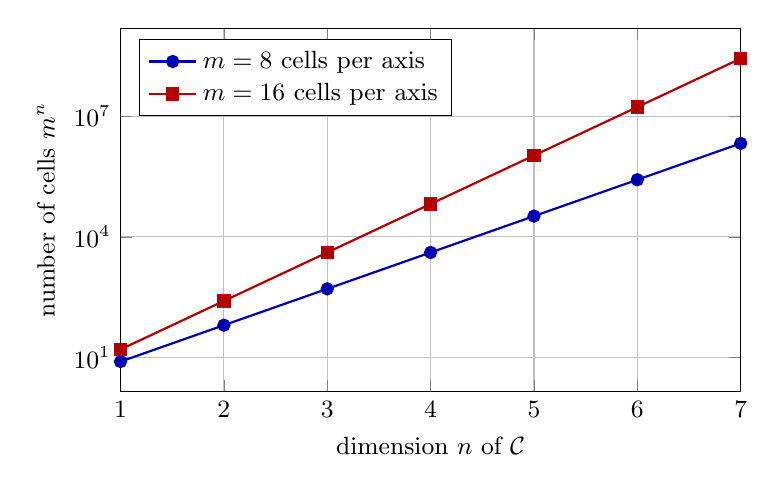
\begin{tikzpicture}
\begin{axis}[width=0.78\textwidth,height=6.2cm,xlabel={dimension $n$ of $\Cspace$},ylabel={number of cells $m^n$},
  ymode=log,xmin=1,xmax=7,xtick={1,...,7},grid=both,legend pos=north west,legend cell align=left,
  tick label style={font=\small},label style={font=\small},legend style={font=\small}]
\addplot[blue!70!black,thick,mark=*] coordinates {(1,8)(2,64)(3,512)(4,4096)(5,32768)(6,262144)(7,2097152)};
\addlegendentry{$m=8$ cells per axis}
\addplot[red!70!black,thick,mark=square*] coordinates {(1,16)(2,256)(3,4096)(4,65536)(5,1048576)(6,16777216)(7,268435456)};
\addlegendentry{$m=16$ cells per axis}
\end{axis}
\end{tikzpicture}
\caption{Why cell-based methods do not scale: a uniform decomposition with $m$ cells per axis has $m^n$ cells in an $n$-dimensional $\Cspace$. Doubling the resolution multiplies the cost by $2^n$.}
\label{fig:scaling}
\end{figure}

\paragraph{Key take-aways.}
\begin{itemize}
  \item Motion planning is naturally formulated in $\Cspace$, where the robot is a point and obstacles are inflated into $\Cspace$-obstacles; $\Cfree$ may be disconnected, and a planner must return a safe path or a failure.
  \item For a translating rigid robot $\CO_i=\Obs_i\Mink(-\Rob_0)$ (isotropic for a disk, anisotropic for polygons); with rotation, slices are stacked; for manipulators, $\Cspace$-obstacles need inverse kinematics and may merge or disconnect $\Cfree$.
  \item The retraction method reduces planning to a graph search on the generalized Voronoi diagram, the maximum-clearance roadmap: complete, multiple-query, $O(v\log v)$.
  \item Exact cell decomposition (sweep-line, convex cells) has the same guarantees but produces a \emph{channel} of paths, flexible enough for nonholonomic constraints or unexpected obstacles; approximate decomposition (quadtrees) is only resolution complete and single-query.
  \item All of these methods need $\CO$ and scale exponentially with $\dim\Cspace$, which motivates probabilistic (PRM, RRT) and potential-field methods, which do not need $\CO$.
\end{itemize}

\end{document}